\scanpage{165}

tout décrire en termes de théorie des groupes, \deleted{\unsure{via une s}} \inserted{en termes} d'une structure d'extension (10). Ici on trouve des générateurs canoniques de $G_0$

\[
\left\{\begin{aligned}
 &\tau_0,\tau_1,\tau_\infty\in G_0\qquad\text{satisfaisant}\\
 &\deleted{\unsure{\tau_1|P_1}}\rho_1^{2}=\rho_\infty^3=1\qquad\text{où }\rho_1=\tau_0\tau_\infty,\ \rho_\infty=\tau_1\tau_0,\\
 &\hspace{13em}\rho_0=\tau_\infty\tau_1
\end{aligned}\right.\tag*{(21)}
\]

si $n$ est l'ordre de $\rho_0$ (il sera fini dans les cas les plus intéressants) on aura donc aussi

\[ \rho_0^n=1,\tag*{(22)} \]

$n$ sera aussi l'ordre des sommets du graphe régulier $\Gamma_0=(S,A_0)$, i.e. du 2-polyèdre régulier $P_0$. Il faut interpréter $S$ comme espace homogène sous $G$, via l'origine $s_0\in S$, donc il faut travailler avec le stabilisateur

\[ G_{s_0}=\{g\in G\mid gs_0=s_0\}=B' \tag*{\deleted{\unsure{(23)}}} \]

dont l'intersection avec $G_0$ sera donné par

\[
\begin{aligned}
B'\cap G_0&=\text{sous-groupe }\inserted{\widetilde U}\ \text{engendré}\text{ par }\tau_1,\tau_\infty\\
 &\hspace{1em}\text{(isomorphe à }\unsure{\mathbb D|D|\mathbf D}_n\text{)}
\end{aligned}\tag*{\deleted{\unsure{(24)}}}
\]

on a donc

\[
\begin{aligned}
G/B'&\stackrel{\sim}{\text{---}}S\\
g.B'&\mathrel{\unsure{\vdash\!\!-\!\dashv|\longmapsto}}g.s_0
\end{aligned}\qquad\substack{\text{isom d'espaces}\\\text{homogènes}\\\text{sous }G}\tag*{\deleted{\unsure{(25)}}}
\]

\figure{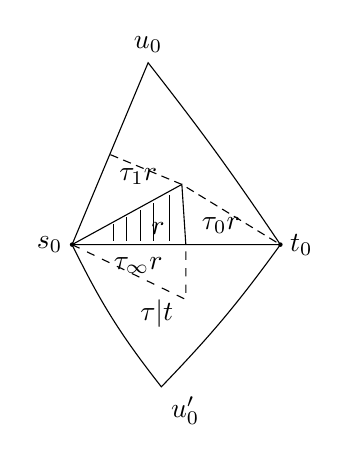
\begin{tikzpicture}[x=1cm,y=1cm,scale=.84]
\coordinate (s) at (0,0); \coordinate (t) at (3.15,0); \coordinate (u) at (1.15,2.75); \coordinate (v) at (1.35,-2.15);
\coordinate (c) at (1.66,.91); \coordinate (b) at (1.72,-.83);
\draw (s)--(u) to[bend left=2] (t)--(s) to[bend right=6] (v) to[bend right=4] (t);
\draw[densely dashed] (.58,1.36)--(c)--(t); \draw (s)--(c)--(1.72,0);
\draw[dashed] (s)--(b)--(1.72,0);
\foreach \x in {.62,.82,1.03,1.23,1.47}{\draw[thin] (\x,.06)--(\x,{.51*\x});}
\fill (s) circle (.034) (t) circle (.034);
\node[left] at (s) {$s_0$}; \node[right] at (t) {$t_0$}; \node[above] at (u) {$u_0$}; \node[below right] at (v) {$u'_0$};
\node at (1.3,.24) {$r$}; \node at (1,1.03) {$\tau_1 r$}; \node at (2.25,.29) {$\tau_0 r$}; \node at (1,-.31) {$\tau_\infty r$}; \node at (1.28,-1.05) {$\unsure{\tau|t}$};
\end{tikzpicture}}

% archive sheet number: 164
